\capitulo{4}{Técnicas y herramientas}

% Este capítulo recoge las técnicas metodológicas y herramientas utilizadas para el desarrollo del proyecto \textit{Asistente de prácticas ágiles para repositorios en GitHub}, así como las decisiones tomadas en función de las alternativas disponibles. La elección de las tecnologías ha estado guiada tanto por los requisitos funcionales del sistema como por los objetivos técnicos y personales planteados.

\section{Metodología de desarrollo}

Durante el desarrollo del proyecto se ha seguido un enfoque iterativo e incremental, inspirado en las metodologías ágiles, especialmente en la metodología \textbf{Scrum}. Aunque no se ha implementado un Scrum completo con sprints y reuniones formales, sí se ha adoptado la filosofía de desarrollo en pequeñas iteraciones, con validaciones frecuentes de funcionalidad y mejora continua.

Cada iteración se centraba en funcionalidades concretas: la recolección de datos, la visualización de medidas de proceso, el cumplimiento de las prácticas ágiles y la mejora de la experiencia de usuario. Esta división permitió avanzar progresivamente, validando en cada iteración los resultados parciales antes de pasar a la siguiente.

Además, se ha hecho uso de herramientas como \textbf{Zube} para la organización de tareas y la planificación de Issues. Esto ha facilitado el seguimiento del progreso del desarrollo.

\begin{figure}[H]
\centering
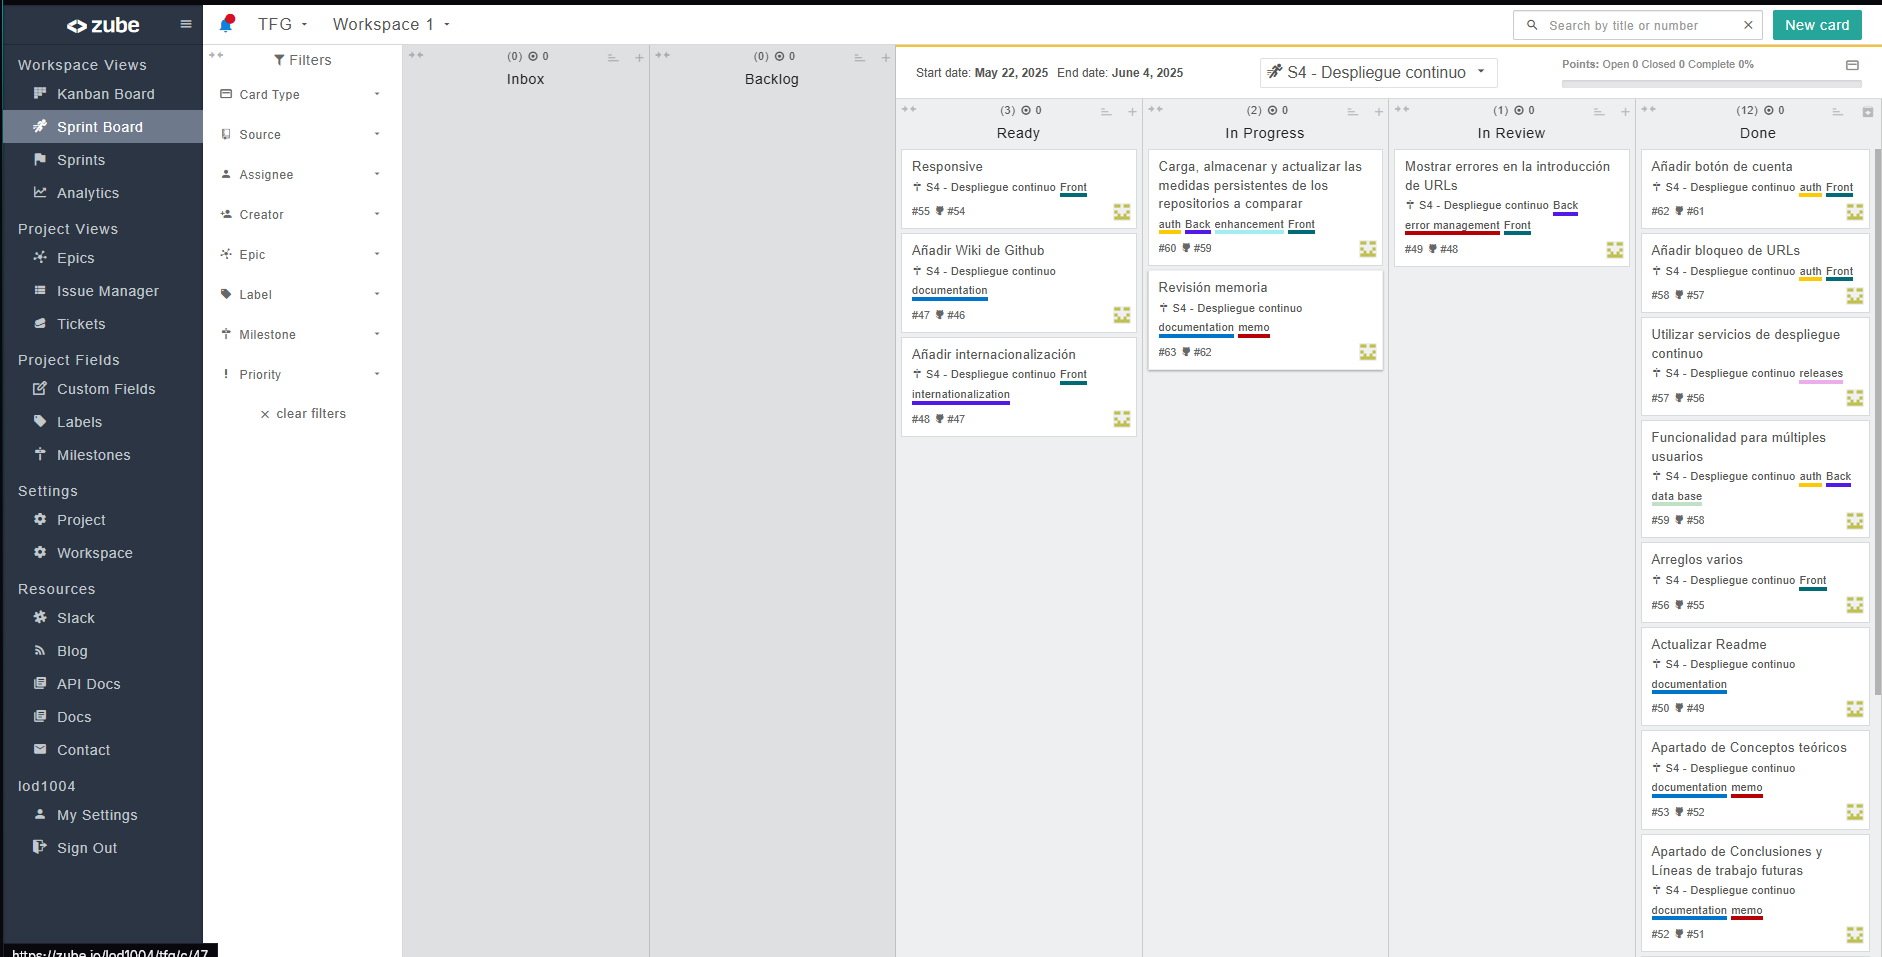
\includegraphics[width=0.8\textwidth]{img/IteracionZube.png}
\caption{Tablero Kanban de la herramienta Zube utilizada para la planificación de tareas e iteraciones.}
\label{fig:zube}
\end{figure}

\section{Tecnologías y herramientas utilizadas}

\subsection{Frontend: Angular}

Para la implementación del cliente se ha optado por el framework \textbf{Angular}, en su versión 19.2.3. Angular ofrece una arquitectura basada en componentes, módulos reutilizables, servicios inyectables y soporte integrado para formularios reactivos. Algunas de sus características más destacadas y útiles en este proyecto han sido:

\begin{itemize}
  \item Formularios reactivos con validación dinámica.
  \item Módulos reutilizables para organizar mejor el código.
  \item Inyección de dependencias para desacoplar lógica y facilitar pruebas.
  \item Integración con bibliotecas como Angular Material para las interfaces de usuario.
\end{itemize}

Se consideraron otras opciones como \textbf{React}, pero se optó por Angular debido a su enfoque más completo y estructurado, más adecuado para una aplicación de análisis con múltiples pantallas y lógica interna, además de la existencia de experiencias previas adquiridas durante las prácticas en empresa en Softeca.

\subsection{Backend: Node.js}

Para el backend se ha utilizado \textbf{Node.js}, un entorno de ejecución para JavaScript que permite desarrollar aplicaciones del lado del servidor de manera eficiente y escalable. Se ha estructurado el servidor como una API REST que recibe peticiones desde el cliente Angular, procesa los datos y devuelve los resultados del análisis.

\begin{itemize}  
  \item \textbf{Modularidad y ecosistema}: Se han utilizado módulos como \texttt{express} para la definición de rutas y controladores, y bibliotecas específicas para consumir APIs de GitHub y procesar datos.
  
  \item \textbf{Facilidad de integración}: Al estar escrito en JavaScript, el backend se integra de forma natural con el frontend desarrollado en Angular, facilitando la comunicación y compartición de lógica o estructuras comunes, lo que facilita el desarrollo.
  
  \item \textbf{Manejo eficiente de errores y validaciones}: Se ha implementado una estructura de control de errores robusta, validación de parámetros de entrada, y respuestas claras al cliente ante peticiones incorrectas o fallos del análisis.
\end{itemize}

Se consideraron otras alternativas como Python (con frameworks como FastAPI o Flask), pero se optó por Node.js por su rapidez de desarrollo, la familiaridad con el lenguaje y su amplia adopción en aplicaciones web modernas.

\subsection{Comunicación cliente-servidor}

La comunicación entre el cliente Angular y el backend FastAPI se realiza a través de peticiones HTTP RESTful, usando el módulo \texttt{HttpClient} de Angular. La respuesta del backend incluye las medidas de proceso en los repositorios a analizar y a evaluar a partir de los repositorios de referencia proporcionados por el usuario.

\subsection{Base de datos: MongoDB y MongoDB Compass}

Para el almacenamiento de información relacionada con los análisis realizados y la persistencia de datos relevantes, se ha utilizado \textbf{MongoDB}, una base de datos NoSQL orientada a documentos. Esta elección se debe a su flexibilidad, escalabilidad y facilidad de uso con Node.js.

\begin{itemize}
  \item \textbf{Modelo de documentos}: MongoDB permite trabajar con documentos en formato JSON, lo cual se adapta perfectamente a los datos semiestructurados obtenidos del análisis de los repositorios de GitHub.
  
  \item \textbf{Integración con Node.js}: Se ha utilizado la biblioteca \texttt{mongoose} para gestionar la conexión, definición de esquemas y operaciones con la base de datos desde el backend Node.js, facilitando el trabajo con modelos y validaciones.
  
  \item \textbf{Visualización y gestión con MongoDB Compass}: Para la gestión visual y análisis manual de los datos almacenados se ha utilizado \textbf{MongoDB Compass}, una interfaz gráfica que permite explorar documentos, ejecutar consultas, y visualizar estadísticas de uso de la base de datos de forma sencilla e intuitiva.
  
\end{itemize}

La elección de MongoDB frente a bases de datos relacionales como MySQL o PostgreSQL se justifica por la naturaleza no estructurada de los datos analizados y la necesidad de una estructura flexible que pueda evolucionar fácilmente sin migraciones complejas, además se su buena integración con el backend Node. js.


\subsection{Diseño de la interfaz de usuario}

Se ha utilizado la biblioteca \textbf{Angular Material} para implementar una interfaz moderna y coherente visualmente. Esta biblioteca proporciona componentes reutilizables (botones, tablas, inputs, spinners, etc.) con accesibilidad integrada y estilos basados en Material Design.

El diseño se ha centrado en la claridad y la simplicidad, mostrando los resultados del análisis de manera visual e intuitiva, junto con retroalimentación clara (colores, iconos, puntuaciones) para ayudar al usuario a interpretar los resultados.

\subsection{Gestión del código fuente}

El código fuente del proyecto se ha gestionado con \textbf{Git}, utilizando GitHub como repositorio remoto. Se ha trabajado con ramas para separar funcionalidades y mantener el código estable en la rama principal.

\subsection{Despliegue continuo de la aplicación web durante el desarrollo}

Para las pruebas de aceptación del tutor y el desarrollo del proyecto se han utilizado dos herramientas: Render y Vercel. Estas herramientas han permitido el despliegue continuo de la aplicación web a través de la integración continua lograda gracias a la compatibilidad entre estas dos herramientas y el repositorio de GitHub donde se ha ido subiendo el código del backend y el frontend

\begin{itemize}
  \item \textbf{Despliegue continuo del backend}: Se ha utilizado la herramienta de Render para lograr el despliegue continuo del backend desde el repositorio de GitHub
  
  \item \textbf{Despliegue continuo del frontend}: Para el frontend se ha utilizado la herramienta de Vercel, que permite un despliegue continuo rápido y eficiente, que se puede probar desde cualquier dispositivo por cualquier persona gracias a la opción de usar despliegues de carácter público.
  
\end{itemize}

Estas herramientas de despliegue han mejorado la comunicación y las pruebas de aceptación tanto al tutor como a diferentes usuarios que han ayudado al desarrollo de la aplicación web y a la búsqueda de errores.

\section{Otras herramientas de apoyo}

\begin{itemize}
  \item \textbf{Visual Studio Code}: Editor principal usado para escribir tanto el frontend como el backend.
  \item \textbf{LaTeX}: Utilizado para la redacción de esta memoria, por su capacidad de estructurar documentos técnicos de manera clara y profesional.
  \item \textbf{Zube}: Para documentar el código, organizar las tareas de desarrollo y las decisiones técnicas dentro del propio repositorio se ha utilizado la herramienta de Zube, recomendada por el profesor y conectada con el repositorio de GitHub.
  \item \textbf{GitHub Desktop}: Herramienta gráfica de GitHub que permite visualizar claramente los cambios realizados en todo el repositorio de forma individual y comparativa antes de subir todos los cambios con un solo Commit.
  
\end{itemize}

\section{Comparativa de tecnologías evaluadas}

Durante la fase inicial del proyecto se analizaron distintas tecnologías. Las siguientes tablas resume los principales aspectos que se compararon:

\begin{center}
\begin{tabular}{|l|c|c|c|}
\hline
\textbf{Tecnología} & \textbf{Facilidad de uso} & \textbf{Rendimiento} & \textbf{Documentación} \\
\hline
Angular & Alta & Media-Alta & Muy completa \\
React & Media & Alta & Muy completa \\
Vue & Alta & Media & Buena \\
FastAPI & Alta & Alta & Muy completa \\
Flask & Alta & Media & Muy completa \\
Django & Media & Media & Muy completa \\
\hline
\end{tabular}
\captionof{table}{Comparativa de tecnologías frontend y backend evaluadas en la fase inicial del proyecto.}
\end{center}

\begin{center}
\begin{tabular}{|l|c|c|c|}
\hline
\textbf{Tecnología} & \textbf{Facilidad de uso} & \textbf{Rendimiento} & \textbf{Documentación} \\
\hline
Node.js & Media-Alta & Alta & Muy completa \\
Express.js & Alta & Alta & Muy completa \\
FastAPI & Alta & Alta & Muy completa \\
Flask & Alta & Media & Muy completa \\
Django & Media & Media & Muy completa \\
Spring Boot & Baja & Muy Alta & Muy completa \\
\hline
\end{tabular}
\captionof{table}{Comparativa de tecnologías backend y frameworks analizados.}
\end{center}


\begin{center}
\begin{tabular}{|l|c|c|c|}
\hline
\textbf{Base de Datos} & \textbf{Facilidad de uso} & \textbf{Rendimiento} & \textbf{Documentación} \\
\hline
MongoDB & Alta & Alto (NoSQL) & Muy completa \\
MySQL & Medio-Alta & Alto & Muy completa \\
PostgreSQL & Media & Muy Alto & Muy completa \\
SQLite & Alta & Medio-Bajo & Buena \\
Firebase Realtime DB & Muy alta & Medio & Buena \\
Redis & Media & Muy Alto (caché) & Buena \\
\hline
\end{tabular}
\captionof{table}{Comparativa de tecnologías de bases de datos utilizadas y evaluadas.}
\end{center}


La elección final se basa en la compatibilidad entre tecnologías, la curva de aprendizaje, y el tipo de aplicación (analítica, con formularios complejos y visualización estructurada).

\section{Resumen de herramientas utilizadas}

A continuación se muestra una tabla con las herramientas utilizadas durante el proceso de desarrollo de software del proyecto, junto con la indicación de a qué parte del proceso corresponden

\begin{table}[H]
\centering
\caption{Herramientas y tecnologías utilizadas en cada parte del proyecto.}
\label{herramientasportipodeuso}
\begin{tabular}{l c c c c c}
\toprule
\textbf{Herramientas} & Frontend & Backend & Base de Datos & Documentación & Despliegue \\
\midrule
HTML5 & X & & & & \\
TypeScript & X & & & & \\
Angular 19.2.3 & X & & & & \\
Node.js & & X & & & \\
XP & & X & & & \\
GitHub API & & X & & & \\
Mongoose & & X & X & & \\
MongoDB & & & X & & \\
MongoDB Compass & & & X & & \\
JWT & & X & & & \\
Render & & X & & & X \\
Vercel & X & & & & X \\
\LaTeX{} & & & & X & \\
Overleaf & & & & X & \\
Git & X & X & X & X & X \\
\bottomrule
\end{tabular}
\end{table}